\documentclass[a4paper, 12pt, twoside]{article}
\usepackage[utf8]{inputenc}
\usepackage[T1]{fontenc}
\usepackage[french]{babel}
\usepackage{graphicx}
\usepackage[hidelinks]{hyperref}
\usepackage[toc,page]{appendix}
\usepackage{float}
\usepackage{amsmath}
\usepackage{fancyhdr}
\pagestyle{fancy}

\fancyhf{}
\fancyfoot[LO]{RedSquare \: 
\includegraphics[scale=0.08]{./TitlePage/ufr}}
\fancyfoot[RE]{
\includegraphics[scale=0.08]{./TitlePage/ufr}  \: RedSquare}
\fancyfoot[LE,RO]{\thepage}
\renewcommand\headrulewidth{0pt}
\renewcommand{\footrulewidth}{0.4pt}

\graphicspath{{./Pictures/}}

\begin{document}

\begin{titlepage}
\begin{center}


\includegraphics[scale=0.50]{./TitlePage/LOGOST}~\\[1cm]

\textsc{\LARGE UFR Sciences et Techniques  Besançon}\\[1.5cm]
Rapport\\
\textsc{Projet de Licence}

\newcommand{\HRule}{\rule{\linewidth}{0.5mm}}

\HRule \\[0.4cm]

{\huge \bfseries RedSquare}

\HRule \\[1.5cm]

\end{center}
\begin{minipage}{0.9\textwidth}
\begin{center} \large

\textsc{Lucas Grosjean, }
\textsc{Rémi Simonin, }
\textsc{Vincent Tourneret}
\textsc{et Florian Vetter}
\end{center}
\end{minipage}
\newline

\begin{center} \large
Tuteur de projet\\
\textsc{Julien Bernard}
\end{center}

\vfill

\begin{center}
{\large \today}
\end{center}

\end{titlepage}

\newpage
\section*{Introduction}
\textbf{Un roguelike} est un jeu vidéo de type RPG ( \textit{Role Playing Game} ). D'un point de vue historique, le premier jeu de la lignée se nomme \textbf{Rogue}. Né en 1980, il donne lieu à plusieurs dizaines de successeurs qui ont repris les codes du genre. L'objectif principal de ce type de jeu est de parcourir un donjon le plus longtemps possible et de ne pas mourir sous les coups des monstres rencontrés.\par
Les roguelike sont définis par certaines caractéristiques, comme la génération procédurale, un système de tour-par-tour et une absence de sauvegarde.\par
Afin de présenter notre version du roguelike, nous expliquerons dans une première partie les règles du jeu. Nous parlerons des différentes interactions qu'un utilisateur peut avoir avec le système ainsi que l'utilisation des classes au sein de celui-ci. Nous poursuivrons dans une deuxième partie avec nos implémentations ainsi que de nos choix techniques. Nous finirons par une troisième partie qui expliquera notre ressenti sur le projet ainsi que notre organisation de travail en groupe. 
\newpage
\tableofcontents
\newpage
\section{Spécifications et modélisation}

\subsection{Règles du jeu}
Au début d'une partie, le joueur a le choix entre 5 classes de personnages. Il ne peut pas changer en cours de jeu. Le nombre de joueurs pour une instance de jeu est compris entre 1 et 9. Plusieurs personnages de même classe peuvent être utilisés. Voir table \ref{perso}
\begin{table}[h]
\begin{center}
\begin{tabular}{  c  }
    
\includegraphics[scale=3]{Players/Magus}
    
\includegraphics[scale=2.2]{Players/WarriorNew} 
    
\includegraphics[scale=2.2]{Players/Rogue} 
    
\includegraphics[scale=2.2]{Players/Ranger} 
    
\includegraphics[scale=2.2]{Players/Healer}
\end{tabular}
\caption{Les Personnages}
\label{perso}
\end{center}
\end{table}
Lorsque la partie débute, tous les joueurs sont niveaux 1. Il n'existe pas de système de sauvegarde. Les tours de jeu sont définis par l'ordre d'arrivée des joueurs dans la partie. Une notification prévient la personne quand c'est à elle de jouer.\\\par
Le joueur a deux choix d'actions par tour. Il peut se déplacer en utilisant les flèches directionnelles, les touches z,q,s,d ou la souris. Celle-ci est le seul moyen de choisir une destination ne se trouvant pas sur les cases adjacentes à la position actuelle. Le chemin choisi est visible par un système de surbrillance. Si la case choisie n'est pas une case sur laquelle nous pouvons nous déplacer alors l'action n'est pas déclenchée. Le joueur est alors obligé de choisir une nouvelle destination, une autre action. Il peut également passer son tour. Voir figure \ref{Chemin}
\begin{figure}[H]
    \begin{center}
	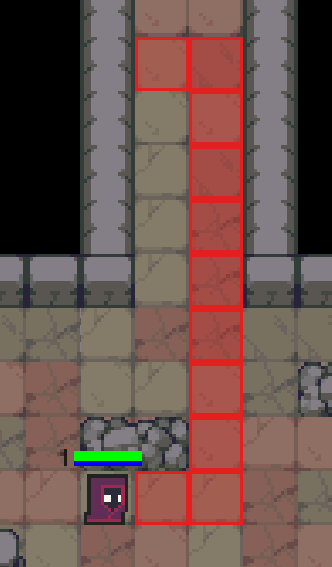
\includegraphics[scale=0.3]{GraphiqueInGame/CheminSelection}
	\caption{Chemin}
	\label{Chemin}
	\end{center}
\end{figure}
 Si un ennemi se trouve à proximité, l'utilisateur peut le pointer avec sa souris. Si le curseur ne prend pas la forme d'une épée, c'est que le monstre ne se trouve pas dans l'aire de combat du personnage. Le joueur a le choix entre une attaque de base, que toutes les classes possèdent dès le départ, ou une attaque spéciale propre à chaque classe. Ces attaques consomment du mana. Celui-ci permet de ne pas abuser des sorts puissants. Une fois le mana épuisé, il faudra changer de niveau ou prendre une potion adéquate afin de le récupérer.\\\par
Chaque personnage peut attaquer à une distance différente selon son type de classe. Par exemple, le guerrier pourra attaquer uniquement les ennemis se trouvant sur les cases adjacentes tandis que le mage pourra attaquer à 2 cases autour de lui.
Certains ennemis sont plus difficiles à vaincre que d'autres. Il est donc important ne pas se précipiter et anticiper les attaques afin de perdre le moins de vies possible. Voir table \ref{monster}\par
\begin{table}[H]
\begin{center}
\begin{tabular}{  c  }
    
\includegraphics[scale=2]{Monsters/Bat}
    
\includegraphics[scale=2]{Monsters/Demon} 
    
\includegraphics[scale=2]{Monsters/Goblin} 
    
\includegraphics[scale=2]{Monsters/Imp} 
    
\includegraphics[scale=2]{Monsters/LilGob}
    
\includegraphics[scale=2]{Monsters/LilZombie}\\
    
\includegraphics[scale=2]{Monsters/Lizard}
    
\includegraphics[scale=2]{Monsters/Mud}
    
\includegraphics[scale=2]{Monsters/Orc}
    
\includegraphics[scale=2]{Monsters/Shaman}
    
\includegraphics[scale=2]{Monsters/SkeletonKnife}\\
    
\includegraphics[scale=2]{Monsters/SkeletonMagus}
    
\includegraphics[scale=2]{Monsters/Slime}
    
\includegraphics[scale=2]{Monsters/Spirit}
    
\includegraphics[scale=2]{Monsters/Swamp}
    
\includegraphics[scale=2]{Monsters/Zombie}
\end{tabular}
\caption{Les Monstres}
\label{monster}
\end{center}
\end{table}
Si un coffre se trouve à proximité, l'utilisateur peut l'ouvrir et glisser les objets dans son inventaire. Pour savoir si le coffre s'ouvre, une clé remplace le curseur actuel. Cette action ne met pas fin au tour du joueur. Voir figure \ref{inventaire}\\\par
\begin{figure}[H]
    \center
	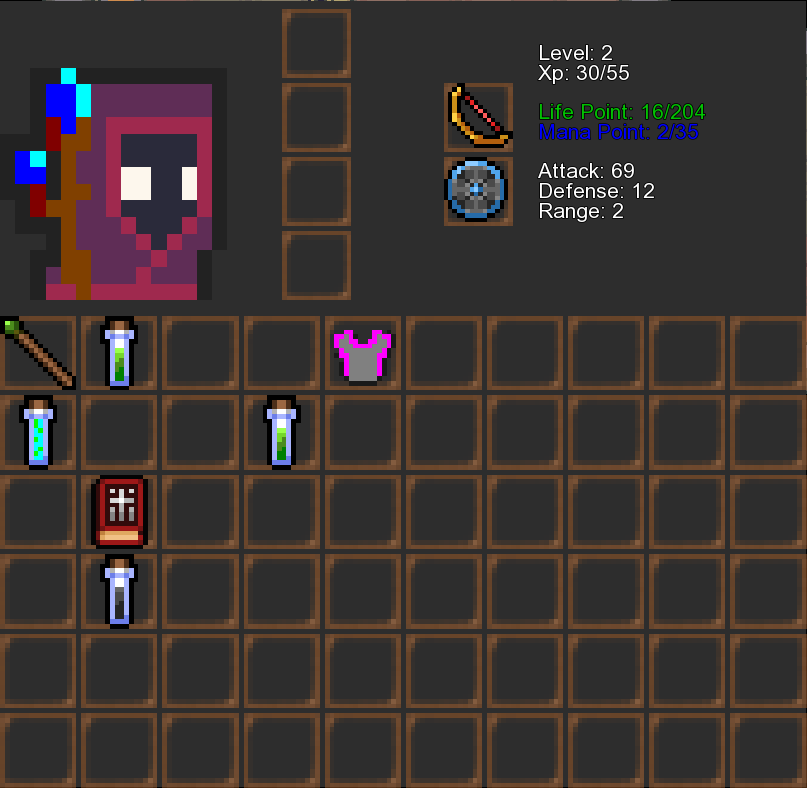
\includegraphics[scale=0.3]{Inventaire}
	\caption{Inventaire}
	\label{inventaire}
\end{figure}
Un joueur peut effectuer certaines actions même si ce n'est pas son tour. Ces actions sont possibles à tout moment.\par
Il peut tout d'abord utiliser son inventaire. Pour l'ouvrir il faut appuyer sur la touche "i". Il peut alors s'équiper d'armes ou d'armures qui augmentent ses performances. Il est aussi capable d'utiliser des potions qui lui augmenteront redonneront de la vie ou/et du mana ainsi qu'une amélioration d'attaque ou de défense.\\\par
L'utilisateur peut également afficher la Mini-map en appuyant sur la touche "m". Celle-ci rendra compte de la disposition de l'étage ainsi que la position de ses équipiers. Voir figure \ref{minimap}\\\par
\begin{figure}[H]
    \center
	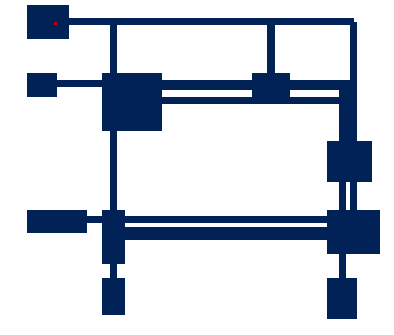
\includegraphics[scale=1]{Mini-Map}
	\caption{Minimap}
	\label{minimap}
\end{figure}
Le joueur peut communiquer avec ses coéquipiers en utilisant le chat. Il a le choix d'envoyer des messages globaux, pouvant être lus par tous, ainsi que des messages privés, destinés à un unique équipier. Le chat permet également de tenir compte de l'avancement du jeu. Les messages provenant du système affichent les précédentes actions de la partie. Par exemple, la mort d'un adversaire sera visible par tous les joueurs. Voir figure \ref{chat}\\\par
\begin{figure}[H]
    \center
    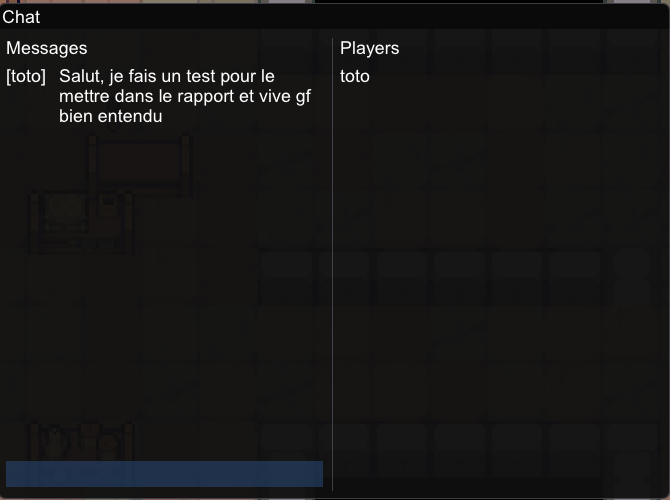
\includegraphics[scale=0.5]{Chat}
    \caption{Chat}
    \label{chat}
\end{figure}    
L'utilisateur à la possibilité de lancer une partie quand il le veut. Il peut également se trouver dans plusieurs parties à la fois.
\newpage
\subsection{Représentation UML}
\begin{figure}[H]
    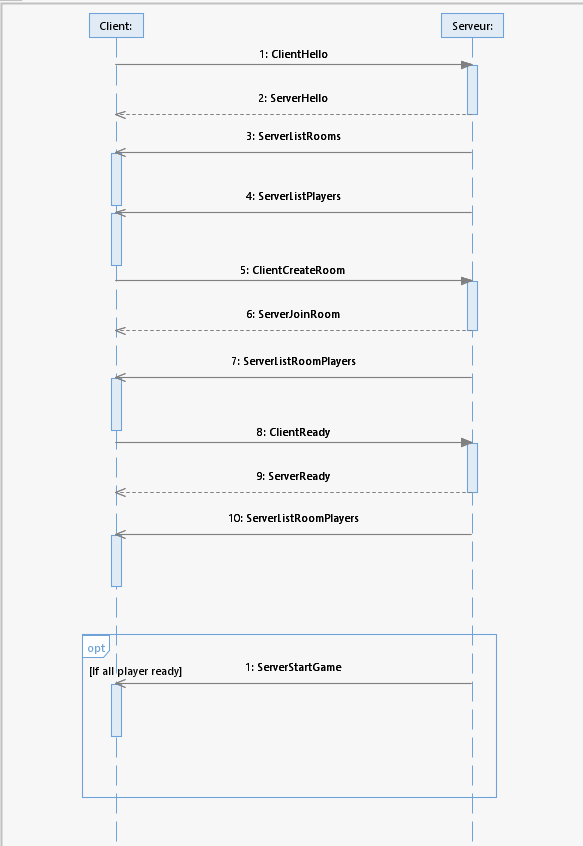
\includegraphics[scale=0.6]{./Diagramme/Connection}
    \caption{Protocole de connexion}
\end{figure}
\newpage
\begin{figure}[H]
    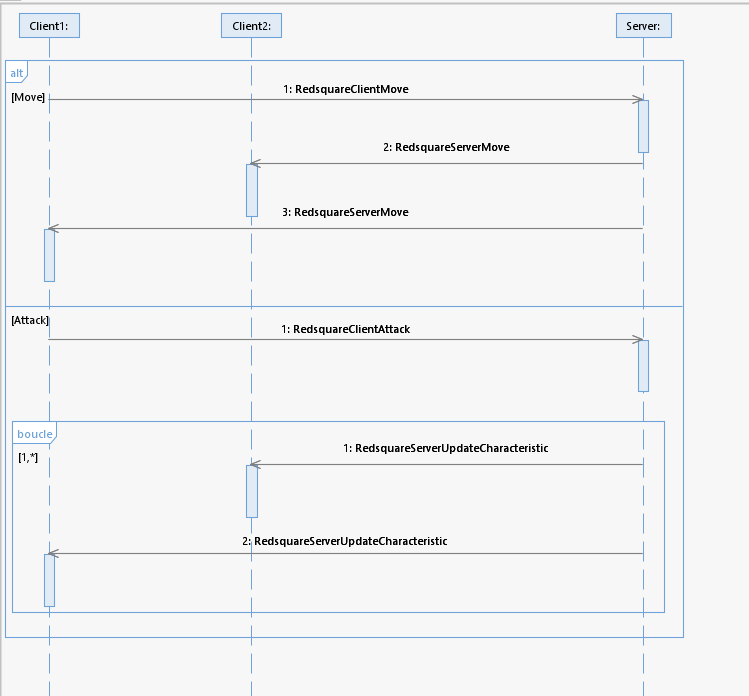
\includegraphics[scale=0.65]{./Diagramme/Deplacement}
    \caption{Protocole de déplacement et de combat}
\end{figure}
Lorsqu'un joueur fait un déplacement, il envoie le paquet "RedsquareClientMove" qui contient un vecteur, qui permet de savoir la direction du déplacement, le serveur regarde si les conditions sont toutes correctes, si c'est le cas, le serveur envoie à tous les joueurs le paquet "RedsquareServerMove" avec le type d'entité, l'id de celui-ci et la position.
Lorsqu'un joueur fait une attaque, il envoie le paquet "RedsquareClientAttack" qui contient un vecteur, qui permet de savoir la position où l'attaque est destinée et le type de spell utilisé, le serveur regarde si les conditions sont toutes correctes, si c'est le cas, le serveur envoie à tous les joueurs le paquet "RedsquareServerUpdateCharacteristic" avec le type d'entité, l'id de celui-ci et toutes ses caractéristiques.
\newpage
\begin{figure}[H]
    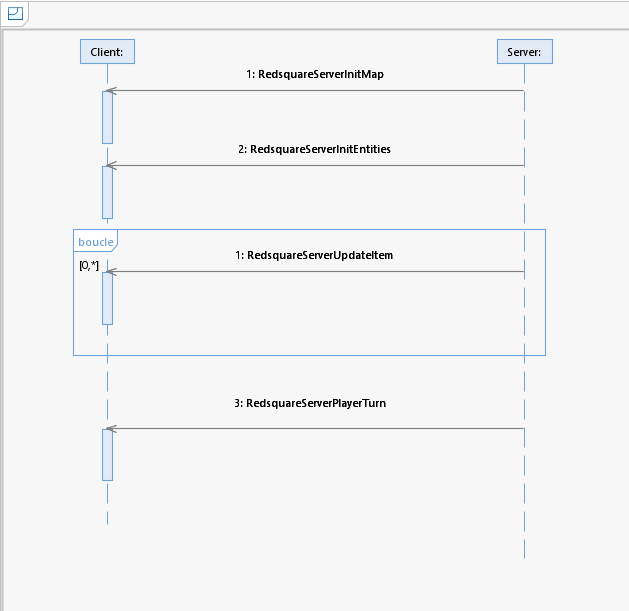
\includegraphics[scale=0.65]{./Diagramme/Jeu}
    \caption{Protocole d'initialisation du jeu}
\end{figure}
Lors de la connexion, Nous devons d'abord envoyer la carte à tous les joueurs grâce au paquet RedsquareServerInitMap. Ensuite nous devons envoyer toutes les entités créées au préalable lors de la génération dans le paquet "RedsquareServerInitEntities", qui contient un vecteur de structure qui contient toutes les donnés pour la création de l'entité. Ensuite nous envoyons tous les items créés dans les différents objets de la carte avec le paquet "RedsquareServerUpdateItem". Et pour finir, nous envoyons le paquet "RedsquareServerPlayerTurn" au premier joueur qui doit jouer son tour.
\newpage
\begin{figure}[H]
    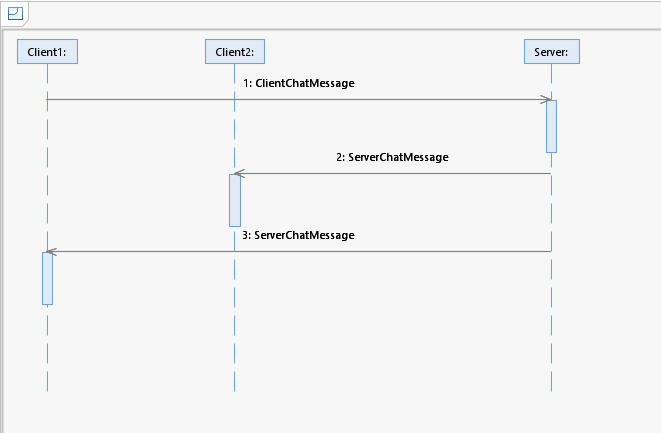
\includegraphics[scale=0.7]{./Diagramme/Chat}
    \caption{Protocole d'envoie d'un message}
\end{figure}
Lorsqu'un client envoie un message dans le chat, on envoie le paquet "ClientChatMessage" qui contient le message et aussi l'id du destinataire lors d'un message privé. Lorsque le serveur reçoit ce paquet, il envoie le paquet "ServerChatMessage" à tous les joueurs y compris l'envoyeur. Si c'était un message privé, seulement l'envoyeur et le destinataire recevrait le paquet.
\newpage
\subsection{Éléments de gameplay}
\subsubsection{Personnages jouable}
\begin{table}[H]
    \begin{center}
    \begin{tabular}{ | c | c | c | }
    	\hline
        Sprite & Nom & Particularités\\
        \hline
        
        
\includegraphics[scale=2.2]{./Players/Magus} & Mage & Portée de deux cases et dégats moyen\\
        \hline
        
        
\includegraphics[scale=1.9]{./Players/WarriorNew} & Guerrier & Vie et défense élévés\\
        \hline
        
        
\includegraphics[scale=2.2]{./Players/Rogue} & Assasin & Dégats élevés mais peu de défense\\
        \hline
        
        
\includegraphics[scale=2.2]{./Players/Ranger} & Tireur & Portée de trois cases mais peu de dégats\\
        \hline
        
        
\includegraphics[scale=1.9]{./Players/Healer} & Prêtre & Portée de deux cases et soins élevés\\
    	\hline
    \end{tabular}
    \caption{Caractéristiques des personnages}
    \label{perso}
    \end{center}
\end{table}
\subsubsection{Ennemies}

\begin{table}[H]
    \begin{center}
    \begin{tabular}{ | c | c | c | }
    	\hline
        Sprite & Nom & Particularités\\
    	\hline
        
\includegraphics[scale=2]{./Monsters/Orc} 
\includegraphics[scale=2]{./Monsters/Mask}
        
\includegraphics[scale=1.5]{./Monsters/SkeletonKnife} 
\includegraphics[scale=2]{./Monsters/Zombie} & Tanks & Vie et défense élévés\\
        
        \hline
        
\includegraphics[scale=2]{./Monsters/Swamp} 
        
\includegraphics[scale=1.4]{./Monsters/Slime}
        
\includegraphics[scale=1.9]{./Monsters/Spirit}
        
\includegraphics[scale=1.7]{./Monsters/Bat} & Esprits & Dégats élevés mais peu de vie\\
       
        \hline
        
\includegraphics[scale=2]{./Monsters/Demon}
\includegraphics[scale=2]{./Monsters/Imp}
        
\includegraphics[scale=2]{./Monsters/LilGob}
        
\includegraphics[scale=2]{./Monsters/LilZombie} & Assasins & Dégats élevés mais peu de défense\\
        
        \hline
        
\includegraphics[scale=2]{./Monsters/Lizard}
        \includegraphics[scale=1.5]{./Monsters/SkeletonMagus} 
        \includegraphics[scale=1.5]{./Monsters/Goblin}
        \includegraphics[scale=2]{./Monsters/Shaman} & Mages & Portée de 2 cases mais peu de dégats\\
    	\hline
    \end{tabular}
    \caption{Caractéristiques des ennemies}
    \label{monster}
    \end{center}
\end{table}

\subsubsection{Sorts}
Il existe dix-huit sorts dans le jeu. Il y a plusieurs types de sort, comme des sorts de dégâts, de soin et de boost. \\
Nous allons maintenant vous présenter trois sorts : 

\begin{figure}[h]
    \center
    \includegraphics[scale=2]{./Spell/Basic1}\\
    \caption{BasicAttack}
    \label{fig:BasicAttack}
\end{figure}
La figure \ref{fig:BasicAttack} est l'attaque de base de chacun des personnages, cette attaque ne consomme pas de mana contrairement à tous les autres sorts.

\begin{figure}[h]
    \begin{center}
    \includegraphics[scale=2]{./Spell/Reaper1}\\
    \caption{Reaper}
    \label{fig:Reaper}
    \end{center}
\end{figure}
La figure \ref{fig:Reaper} est un sort de zone qui va permettre à son lancer de taper toutes les cases devant lui, ce sort coûte 7 points de mana.\\

\begin{figure}[h]
    \center
    \includegraphics[scale=7]{./Spell/DoubleStrike1} \\
    \caption{DoubleStrike}
    \label{fig:DoubleStrike}
\end{figure}

La figure \ref{fig:DoubleStrike} est un sort qui va frapper sa cible avec 2 attaques qui font chacune 70\% de dégâts par rapport à l'attaque de base, ce sort coûte 5 points de mana.\\

\subsubsection{Objet}
Il existe dans RedSquare, plus de 135 équipements différents. Ces équipements et potions se trouvent dans les coffres que l'on peut trouver dans les salles du donjon. \\
Un joueur peut s'équiper d'une arme (épée, arc, bâton, livre de sort), d'un bouclier, d'un casque, d'un plastron, d'un pantalon et d'une paire de bottes.
Il existe quinze types de ces pièces d'équipement avec chacune des bonus différents, certaines pièces donneront plus de vie alors que d'autre plus de défense.\\
Chacune de ses pièces d'équipement a le même taux d'apparition dans un coffre, à la différence que tous les types d'équipement ne sont disponibles qu'à partir de certains étages.
Les cinq premiers types d'équipement sont disponibles depuis le début alors que les autres ne sont disponibles qu'à partir de l'étage cinq (pour les cinq prochains types) et l'étage quinze (pour les cinq derniers types). 
\\ \\
Dans RedSquare il y a huit types de potion et chacun de ses types de potion contient trois tiers, plus le tier est élevé plus la potion est efficace.\\

\begin{table}[h]
\begin{center}
    \begin{minipage}{10cm}
        \begin{itemize}
        \item Potion de vie
        \item Potion de mana
        \item Potion d'énergie (vie + mana)
        \item Boost de vie
        \item Boost de mana 
        \item Boost d'attaque
        \item Boost de défense 
        \item Boost d'expérience
        \end{itemize}
    \end{minipage}
    \caption{Les différents type de potion dans RedSquare}
    \end{center}
\end{table}
Tous les tiers ne sont pas disponibles dans les premiers étages, en effet comme pour les équipements, les tiers un et deux sont respectivement disponibles à partir de l'étage cinq et quinze.

\subsubsection{Inventaire}
\begin{figure}[H]
    \center
    \includegraphics[scale=0.3]{./Pictures/Inventaire} \\
    \caption{Inventaire}
    \label{Inventaire}
\end{figure}
Nos joueurs ont aussi à leur disposition un inventaire où ils peuvent stocker tous leurs équipements et potions. La figure \ref{Inventaire} montre l'interface de l'inventaire avec plusieurs items à l'intérieur. On peut aussi voir sur la figure \ref{Inventaire} les statistiques du joueur, ses points de vie, point de mana, et son expérience.

\subsubsection{Chat}
Les joueurs ont aussi la possibilité de communiquer via un chat, ce chat permet d'envoyer des messages à tous les joueurs mais aussi des messages privés. C'est aussi sur ce chat que le serveur affichera les différentes informations liées au combat.

\subsubsection{Salle de boss}
\begin{figure}[H]
    \begin{center}
    \includegraphics[scale=0.2]{./Salle_Boss} \\
    \caption{Salle de boss}
    \label{boss}
    \end{center}
\end{figure}
Tous les quatre étages, les joueurs atterrissent dans une salle de boss, cette salle est caractérisée par un nombre d'ennemis conséquents et d'un bon nombre de coffres. Ces salles ajoutent de la difficulté au jeu mais récompensent le joueur s'il réussit à les passer. On peut voir une de ces salles de boss sur la figure \ref{boss}.

\newpage
\section{Réalisation/Implémentation}

\subsection{Choix des technologies}

\subsubsection{Interface réseau}
Nous avons dû faire un choix pour l'interface réseau que nous allons utiliser. Nous avons deux interfaces en concurrence :\\ \\
\begin{tabular}{ | l | l | l | l | }
    \hline
    \multicolumn{2}{|c|}{Boost.Asio} & \multicolumn{2}{|c|}{\verb!gf::net!}\\
    \hline
    Avantages & Inconvénients & Avantages & Inconvénients\\
    \hline
    Rapidité & Utilisation difficile & Utilisation simple & Lenteur\\
	\hline
	Documentation & Plusieurs threads & Sélecteur de socket & Moins d'aide en ligne\\
	\hline
\end{tabular} \\ \\
Pour comparer la rapidité, nous utilisons un système de benchmark, où on envoie un paquet, et on regarde le temps entre l'envoi et la réception, sur la même machine. Nous constatons que \verb!gf::net! est 360 fois plus lent que Boost.Asio. En revanche, pour l'implémentation de Boost.Asio, il faut faire un thread par connexion. Et en gérant le chat à part de la boucle de jeu, alors il faut encore un thread pour le chat + un thread par joueur. Et on doit créer un thread par partie, pour pouvoir gérer plusieurs parties, car nos sockets sont bloquantes. Alors qu'avec \verb!gf::net!, nous pouvons simplement utiliser un sélecteur de socket. Qui nous permet d'éviter d'avoir des appels bloquants, et de pouvoir gérer facilement plusieurs parties coté serveur.

\subsubsection{Interface graphique}
Il nous a fallu gérer les différentes interfaces
graphiques du jeu. Pour cela nous avons comparé les deux outils possibles que nous avons utilisés dans notre projet.\\

Le premier outil, est une classe nommée UI, apportant un rendu satisfaisant, directement implémentée dans gf elle est facile de compréhension et d'utilisation ce qui nous a fait gagner beaucoup de temps.
Mais cette classe apporte quelques inconvénients, pour notre chat qui utilise UI, le texte affiché
ne se retourne jamais à la ligne, ce qui est vraiment problématique pour les
longs messages. Un autre inconvénient est la taille des fenêtres lors du passage de petit à plein écran, en effet la taille de la fenêtre créée ne change pas alors que celle du jeu changeait.
\\Le second outil, est une bibliothèque nommée Dear ImGui, apportant un rendu visuel vraiment agréable et nous permettant de répondre à tous les inconvénients de UI. Donc un retour à la ligne, un changement de taille de la fenêtre, etc. ImGui offre également bon nombre de fonctions nous permettant un rendu visuel personnalisé(arbres, textWrap...).
Les inconvénients de Dear ImGui, sont que la bibliothèque n'étant pas implémentée directement dans gf, la rendant plus difficile d'utilisation (pour la lier à tout notre jeu) et de compréhension. Il y a aussi le fait qu'il n'est pas possible d'intégrer des images dans la fenêtre utilisant ImGui. Un des plus gros inconvénients de ImGui était que l'on ne peut pas changer la taille du texte dans les fenêtres ce qui nous limite lors du passage en plein écran.\\

Après avoir analysé les avantages et les inconvénients nous avons donc décidé d'utiliser Dear ImGui, pour son aspect visuel qui est de qualité. ImGui nous permet également de résoudre les problèmes de UI et donc de pouvoir créer l'affichage graphique voulu.
\\
Pour aller plus loin, aucune des deux technologies testées ne correspond à ce que l'on voulait faire. Nous étions un peu limités par les bibliothèques mais nous avons réussi à produire quelque chose de correct. L'inventaire a besoin d'un affichage, comportant des images que l'on peut Drag and Drop ce qui ne pouvait pas être réalisé ni avec UI ni avec Dear ImGui.
\newpage

\subsection{Génération du jeu}
\begin{figure}[H]
    \center
    \includegraphics[width=10cm,height=6cm]{./Procedural/void}
    \caption{Carte vide}
    \label{vide}
\end{figure}

\begin{figure}[H]
    \center
    \includegraphics[width=10cm,height=6cm]{/Procedural/grid}
    \caption{Grille}
    \label{grid}
\end{figure}

\begin{figure}[H]
    \center
    \includegraphics[width=10cm,height=6cm]{/Procedural/floor}
    \caption{Génération du sol des salles}
    \label{floor}
\end{figure}

\begin{figure}[H]
    \center
    \includegraphics[width=10cm,height=6cm]{/Procedural/wall}
    \caption{Ajout des murs}
    \label{wall}
\end{figure}

\begin{figure}[H]
    \center
    \includegraphics[width=10cm,height=6cm]{/Procedural/corridor}
    \caption{Ajouts des couloirs}
    \label{corridor}
\end{figure}

\begin{figure}[H]
    \center
    \includegraphics[width=10cm,height=6cm]{/Procedural/stair}
    \caption{Placement des meubles, monstres, escalier et joueurs}
    \label{stair}
\end{figure}

La génération de la carte se déroule en plusieurs étapes: \\

La première étape consiste à dimensionner la zone jouable, c'est-à-dire les bornes de la carte. Dans notre jeu, tous les étages font cent cases par cent cases, comme on peut le voir que la figure \ref{vide}.  \\

La seconde étape consiste à créer une grille sur la carte. Cette grille permet de découper la zone jouable en plusieurs carrées où l'on viendra générer les salles du donjon. Cette grille est visible sur la figure \ref{grid}  \\

La troisième étape est la génération du sol des salles, ceci correspond à la figure \ref{floor}. Nous tirons au sort plusieurs carrés où l'on va générer les salles, la plupart du temps nous générons dix salles dans l'étage. Nous sélectionnons un point au hasard dans le carré choisi pour accueillir une salle puis nous tirons au sort la largeur et la longueur (entre six et vingt-six) de la future salle. Si les bornes de la salle dépassent celles du carré alors nous tirons au sort une longueur et une largeur jusqu'à obtenir une salle qui rentre dans le carré. Nous stockons ensuite ces salles dans un vecteur4u qui stocke les quatre coins des salles générées. Une fois les salles générées nous détruisons la grille. \\

La quatrième étape est celle où l'on va placer les murs autour des salles générées dans l'étape précédente, comme on peut le voir sur la figure \ref{wall}. Pour cela nous utilisons le vecteur4u où nous avons stocké les sols des salles, nous parcourons ensuite une zone qui contient le sol de la salle et toutes les cases adjacentes à ce sol. Nous plaçons ensuite des murs sur les cases adjacentes. Nous stockons les salles dans un autre vecteur4u. \\

La cinquième étape de cette génération procédurale est la génération des couloirs permettant de lier les salles entre elles. Pour ce faire, nous sélectionnons deux salles parmi celles que nous avons générées puis on prend le milieu de ces deux salles qu'on relie grâce à la fonction computeRoute() de GF. Cette fonction implémente l'algorithme A* qui calcule le plus court chemin entre deux points et nous renvoie un vecteur contenant les cases du chemin le plus court. Nous parcourons alors ce vecteur pour y placer des cases de sol. Pour rendre la génération plus proche d'un donjon, nous sélectionnons un point adjacent au milieu de des salles que l'on va relier de la même manière que les deux premiers points. Cela permet d'obtenir des couloirs de deux de large. De la même façon que pour les salles, nous plaçons les murs sur les cases adjacentes aux couloirs que l'on vient de générer. Nous exécutons ce processus jusqu'à l'avoir exécuté notre nombre de salles fois trois, ce qui nous permet d'être sûr d'avoir relié toutes les salles entre elles. La figure \ref{corridor} montre la carte après la génération de tous les couloirs.\\

La dernière étape de notre génération est le placement des éléments de jeu (meubles, monstres, escalier et les joueurs), ses différents éléments se trouvent sur la figure \ref{stair}. Nous parcourons une fois encore notre vecteur de salle et nous tirons au sort un thème. Ce thème nous permet de générer tel ou tel meuble en fonction du thème. Nous avons défini de nombreux thèmes tels que, une prison, une armurerie, une bibliothèque, une salle du trône, une salle avec des boîtes et des vases. Les meubles sont des entités destructibles qui ne possèdent qu'un point de vie. Leurs positions est aléatoire dans la salle, pour cela nous tirons une position dans la salle et nous vérifions que le meuble ne rentre pas en collision avec un autre. \par
Pour placer l'escalier nous tirons au sort une case vide dans une salle aléatoire et et on le place à cette position.
Nous plaçons ensuite les ennemis dans les salles de la même manière que les meubles. Nous tirons au sort les salles où les monstres vont apparaître, puis nous tirons une position vide dans cette salle pour y placer le monstre. \par
De la même manière, nous plaçons les joueurs à une position aléatoire dans une salle aléatoire. Nous faisons juste attention à ce que la salle contient un carré de trois pars trois pour faire apparaître neuf joueurs (Nombre de joueurs maximaux en multijoueur). \par
\newpage
\subsection{Gameplay}

\subsubsection{Personnages}
Pour l'implémentation de la classe "joueur", nous avons fait le choix d'utiliser une seule classe, cela allège l'architecture côté client et côté serveur, de plus cela facilite le stockage des entités car avoir plusieurs classes pour la même structure l'aurait rendu plus complexe à utiliser. Le choix du joueur se fait par le client avant le lancement de la partie. Ce choix est ensuite envoyé au serveur à travers un paquet. Ce paquet sera reçu par le serveur qui utilisera le constructeur de la classe. Il existe un seul constructeur pour la classe "joueur", puisque chaque joueur a les mêmes attributs, il n'y a que les valeurs qui changent. Le constructeur passe la classe choisi par le client dans un switch case, qui va attribuer les valeurs aux membres de la classe. On peut voir tous les personnages sur la table \ref{perso} \\ 
Un joueur possède ses caractéristiques : \\
\begin{table}[h]
\begin{center}
    \begin{minipage}{10cm}
        \begin{itemize}
            \item Point de vie
            \item Point de mana
            \item Point de défense 
            \item Point d'attaque 
            \item Expérience 
            \item Portée d'attaque
        \end{itemize}
    \end{minipage}
\end{center}
\end{table}
En plus des différences de caractéristique, les classes n'ont pas accès à tous les sorts. Par exemple, les classes "Warrior" et "Rogue" ont plutôt des sorts offensifs alors que le "Healer" possède plus de sorts défensifs. Les sorts accessibles par telle ou telle classe sont faits manuellement, c'est-à-dire que nous choisissons la liste des sorts disponibles pour la classe. \par
Toutes les entités de joueurs sont stockées côté client et côté serveur dans une map dont la clé est l'ID de l'entité (ID donnée par GF) et la valeur est l'objet joueur. Cette map nous permet de mettre à jour les données concernant les joueurs et d'accéder rapidement à celles-ci via leurs ID respectif.

\subsubsection{Ennemies}
Les ennemis possèdent les mêmes caractéristiques que les joueurs à la seule différence que ceux-ci n'ont pas de point de mana. Comme pour les joueurs, il n'y a qu'une classe pour gérer tous les monstres. Il y a actuellement 17 monstres dans le jeu, voir table \ref{monster}. Les ennemies ne possèdent pas de sort comme les joueurs, ceux-ci sont seulement dotés d'une attaque de base (la même que les joueurs). Les entités ennemies sont stockées de la même manière que les entités "joueurs", c'est-à-dire dans une map dont la clé est l'ID de l'entité et la valeur est l'objet ennemi. Cette map nous permet aussi de modifier les monstres et de mettre à jour leurs données.

\subsubsection{Sorts}
Il existe dans le jeu, dix-huit sorts, tous ces sorts sont implémentés par une même classe, pour les mêmes raisons qu'énoncées plus haut. Il existe deux types aux vues de l'implémentation, les sorts à cible unique et les sorts de zone (qui peut cibler plusieurs entités). \par
Pour la résolution des sorts à cible unique, le client envoie au serveur le sort qu'il vient de lancer avec sa cible, le serveur exécute la méthode associée au sort reçu puis renvoie un paquet contenant les nouvelles données à tous les joueurs. \par
Pour la résolution des sorts de zone, on envoie seulement la case visée par le client au serveur, le serveur va exécuter la méthode associée et va parcourir l'ensemble des cases du jeu affectées par le sort. Si le serveur détecte une entité ennemie sur une de ces cases, on exécute un traitement spécifique au sort sur cette entité. On envoie ensuite aux clients les nouvelles données grâce à des paquets.

\subsubsection{Meubles}
Nous avons aussi implémenté des meubles, c'est-à-dire des éléments de décor que l'on peut détruire (à l'exception des coffres). Il existe 37 meubles à l'heure actuelle. Tous ces meubles sont implémentés dans une même classe, pour les mêmes raisons que la classe "joueur". Ces meubles sont des éléments de décor qui se place sur une ou plusieurs case(s) en fonction du meuble. Les meubles ne peuvent pas être franchis par les joueurs et doivent d'abord être détruits pour pouvoir marcher sur la case. Les meubles sont considérés comme des entités et sont stockés de la même manière que les autres entités, c'est-à-dire dans une map dont la clé est l'ID de l'entité et dont la valeur est l'entité. Les meubles sont supprimés de la map une fois détruits par un joueur.  \par

\subsubsection{Items}
Les items sont implémentés dans une seule classe, cela nous permet d'éviter d'allouer les différents d'objet, et donc d'éviter les possibles fuites mémoires. Chaque item est définie par un type, un nom, une description, un masque pour les slots compatibles et des caractéristiques. Le type de l'item est une énumération, pour la faciliter d'ajouter un item. Le masque nous permet de définir pour chaque item, dans quel slot il peut être ajouté ou déplacé. Lorsqu'un item est déplacé dans un des slots spéciaux du joueur, alors les caractéristiques de l'item sont ajoutées aux caractéristiques du joueur. Les items sont répartie dans deux maps différentes, une avec les slots spéciaux et une avec les slots de cargaison. Lors du déplacement d'un item, on le supprime de l'ancien slot et on le recrée pour l'ajouter dans le nouveau slot.

\newpage
\subsection{Gestion des éléments graphiques}
Pour utiliser tous nos éléments graphiques(Inventaire, Chat, Map, etc), il nous fallait une classe nous permettant de relier toutes les classes qui affichent des éléments a l'écran. Cette classe est nommée Hud qui permet d'afficher ou non les différents outils implémentés, par le simple appuie sur une touche. Hud contient comme implémentation graphique le texte en brut (affichage de l'étage, H for help, etc) réalisé grâce à \verb!gf::Text!.

\subsubsection{Monde}
Notre monde est constitué de case, chaque case à un type, et chaque type de case à un sprite particulier. Nous utilisons un Tileset, qui est un regroupement de sprite nécéssaire à l'affichage . Notre Tileset contient uniquement des sprites en 16x16, cette taille est un choix artistique car nous trouvions que le style du Tileset correspondait à notre jeu. Pour récupérer l'une des cases sur le Tileset, nous utilisons une fonction de GF pour traduire la position de cette case par un entier, par exemple le sprite de l'escalier est la 327ème case de notre Tileset. Dans notre projet, nous avons préférez-nous concentrer sur le code plutôt que de faire notre propre design de jeu. C'est pour cela que nous avons utilisé un Tileset acheté sur internet (10\$). Ce Tileset comprenait tous les sprites des cases du donjon et les meubles. Nous avons aussi utilisé des images libres de droits pour les sprites de nos joueurs et de nos monstres. 

\subsubsection{Barre de vie et de mana}
Le niveau, la barre de vie et de mana des personnages jouables ainsi que des monstres sont implémentés dans la classe Player ou Monster (coté client). Ces éléments sont réalisés grâce aux classes \verb!gf::RectangleShape! et \verb!gf::Text!. Pour placer les éléments on récupère la position du personnage au quelle on multiple par TileSize moins la taille de nos barres. Pour donner l'impression de "barre remplie" on superpose deux rectangles l'un sur l'autre.Pour donner l'impression de "barre qui se vide" on réduit la barre au premier plan petit à petit.
\begin{figure}[H]
    \begin{center}
    \includegraphics[scale=0.5]{./GraphiqueInGame/BarreVieMana}
    \caption{Barre de vie et de mana}
    \end{center}
\end{figure}

\subsubsection{Inventaire}
La figure \ref{Inventaire} permet de représenter l'inventaire. Le fond de l'inventaire est définie grâce à \verb!gf::UI!, cela nous permet d'avoir un fond. Ensuite chaque slot est défini dans une classe InventorySlot qui contient un \verb!gf::SpriteWidget! pour afficher le fond du slot. Cette classe permet l'affichage du slot, et l'affichage de l'item s'il est présent dans le slot. Cela nous permet de différencier chaque slot. Nous avons pris en compte la taille du widget parent pour pouvoir calculer chaque taille de widget, ce qui nous permet d'avoir un chat réactif par rapport à la taille de la fenêtre du jeu. Lors d'un ajout ou d'une suppression d'un item dans l'inventaire, nous avons un message qui est envoyé à l'interface de l'inventaire. Ce message permet d'ajouter ou d'enlever le pointeur de l'item présent dans le slot. Pour gérer le déplacement d'item, nous utilisons un widget qui suit le pointeur de la souris, lorsque nous avons fait un clique gauche sur un slot. Nous utilisons \verb!gf::Text! pour l'affichage des caractéristiques du personnage lors de l'ouverture de l'inventaire.

\subsubsection{Sorts}
Les spells sont définis côtés serveur dans Player et côtés client dans SpellWidget. SpellWidget contient le nom, l'image, la description et le coût en mana.  L'implémentation de l'affichage ce fait dans Hud, en utilisant \verb!gf::Sprite!. Le premier sort a une position propre définie, à chaque fois que l'on gagne un nouveau sort, la position de celui-ci est égale à la position du précédent + 1,2(horizontalement). Après quatre spells, la position du prochain sort revient à la position du premier + 1,2(verticalement) et les suivants seront sur la même ligne.
Lors du passage de la souris sur un sort, une bulle d'aide générée avec Dear ImGui s'affiche et nous donne les informations définies dans SpellWidget.
\begin{figure}[H]
    \begin{center}
    \includegraphics[scale=0.5]{./GraphiqueInGame/Spells}
    \caption{Exemple de placement des sorts}
    \end{center}
\end{figure}

\subsubsection{Chat}
Le chat en jeu est définie dans GameChat, cette classe contient tout l'affichage du chat en utilisant Dear ImGui. La position du chat est identique que l'on soit en plein écran ou non. Pour sa taille on utilise \verb!gf::Coordinates!, getRelativeSize() et un vecteur2f. On utilise le vecteur2f dans laquelle on ajoute coordinates '.' la fonction getRelativeSize() possédant deux valeurs correspondant à la taille voulue en petit écran. Cela permet que l'affichage soit dynamiquement relié à la taille de la fenêtre et donc selon la taille de la fenêtre celle du chat évolue également. Pour la position la mécanique est la même.
Le chat est séparé en deux, la première moitié est constituée du texte des potentiels messages ainsi que de la zone pour écrire un message. La seconde moitié est constituée d'une zone résumant les utilisateurs présents dans le chat.

\subsubsection{Mini-Map}
La figure \ref{minimap} permet de représenter la mini-map dans notre jeu. On prend la représentation du monde dans une \verb!gf::Array2D! qui contient chaque tile. On l'a parcours, lorsqu'on passe sur un tile différent de void, alors on ajoute un carré dans une \verb!gf::ShapeParticles! représentant cette tile. Si on modifie la taille de la représentation de chaque particule, alors nous pouvons agrandir ou réduire la taille de la mini-map sur l'hud. Ensuite on regarde la position de notre joueur et de nos alliés et on remplace la particule avec une couleur prédéfinie. Cela nous permet d'afficher la position des joueurs sur la mini-map. En utilisant une \verb!gf::ShapeParticles! cela nous permet de réduire le nombre d'appels fait à la carte graphique pour afficher la mini-map, car elle va permettre d'afficher en un seul appel au lieu de plusieurs appels si on aurait utilisé \verb!gf::RectangleShape! pour chaque tile par exemple.

\subsection{Sérialisation}
Afin de faire transiter nos paquets en réseau, nous avons appris à les sérialiser. Cette action consiste à découper un objet en plusieurs petites parties afin de minimiser la perte d'informations et de simplifier le transfert de données. Chaque objet sera transformé en tableau de bytes. Cette transformation est possible via l'utilisation  du système de sérialisation  implémenté dans gf. Voici un exemple simple: si un joueur veut se déplacer, alors il envoie un paquet de déplacement. Celui-ci est composé d'un Vector2i comportant la position en x et la position en y. Le Vector2i est transformé en tableau de bytes. Lorsque le serveur reçoit ce paquet il doit alors le désérialiser. C'est-à-dire qu'il doit reformer le paquet de déplacement en remettant les informations du Vector2i dans le bon ordre.
\newpage
\section{Conclusion}

\subsection{Aspect gestion de projet}
Étant un groupe de quatre et n'ayant pas les mêmes emplois du temps, il nous fallait
mettre en place des solutions pour nous permettre de travailler rapidement et
efficacement. Il nous fallait donc un outil de développement collaboratif nous
permettant de partager notre travail avec les autres. Nous avons fait le choix
d’utiliser github qui est un service web d’hébergement et de gestion de
développement de logiciels. Lié à GitHub Desktop sur nos machines, il était
facile de partager son code avec les autres ou de gérer d’éventuels conflits dans
notre code.\par

Pour communiquer entre nous à distance, nous avons créé un groupe
messenger et un serveur discord. Lorsque nous voulions travailler depuis chez
nous, tout en voulant discuter du projet nous utilisons notre serveur discord.
Il nous permettait de réaliser des séances dîtes "ouijas" (terme que
nous utilisons pour définir nos soirées de codes tard le soir).
Pour pouvoir travailler entre nous côte à côte, nous nous rejoignions dans une salle de TP
lors de notre temps libre ou les mardis soir pendant les séances du dps
(club de jeu vidéo).\par

Lors de rencontres de problème sur notre implémentation ou sur nos
choix techniques, nous dérangions gentiment et régulièrement notre tuteur. Cela nous permettait de
résoudre rapidement nos problèmes. Les réunions étaient importantes et nous
permettaient de faire le point sur notre code et sur les potentiels problèmes ou évolutions du projet.

\subsection{Perspectives d’amélioration}
Comme tout jeu vidéo, nous pouvons ajouter encore beaucoup de piste pour
améliorer la qualité du jeu. Nous pensons notamment à la création de nouveaux personnages, de sorts, d'items et modèle de salle. Nous pourrions ajouter de vrai boss dans les salles afin de créer de
véritables paliers de jeu et ainsi marquer une sorte de progression. De nouveau
éléments de jeu tel que la gestion d'une monnaie ainsi que l'ajout d'une
boutique par étage nous permettrait d’acheter ou vendre des items. Nous avons également envisagé de créer un système de
sauvegarde des scores. Nous avions aussi pensé à ajouter des animations de combat et de mort, mais nous n'avions pas les sprites nécessaires pour les faire. Nous nous sommes donc contenté d'ajouter des animations neutres qui rendent les personnages et les ennemies un peu plus vivants. Nous avons aussi pensé à prendre un nouveau Tileset contenant des images de plus grande qualité, notre Tileset de sprite 16x16 limite un peu les détails du jeu, nous avions pensé à un Tileset de sprite 32x32 ou 64x64. Nous n'avons pas changé de Tileset pour nous concentrer sur l'ajout de fonctionnalité dans le jeu.

\subsection{Synthèse}
Le sujet est un sujet complet, regroupant la majorité des concepts de l'informatique comme le réseau, la génération procédurale ou la programmation orientée objet. Nous avons proposé ce sujet donc il est facile pour nous de se plonger dedans. C'est un projet de longue haleine, qui nous a demandé d'être méthodique et organisé puisque que nous sommes quatre dans notre groupe.\\ 

La collaboration des développeurs a permis de répartir les tâches de manière efficace.
La quantité de code source écrit pour ce résultat est importante, on mesure le projet
à environ 12 000 lignes.\\

Nous avons développé nos connaissances dans le langage C++ et utiliser des logiciels de versionning. Désormais, le développement du code source est plus intuitif, avec une connaissance plus fine de ce qui fonctionne bien et proprement. Nous avons notamment appris à utiliser des bibliothèques comme GamedevFramework et Dear ImGui.\\

Notre utilisation de GamedevFramework, nous a permis de réparer et d'implémenter de nouvelles fonctionnalités dans cette bibliothèque par le biais de pulls requests.\\ 

Nous avons mené à bien ce projet rapidement, ce qui nous a permis d'implémenter plus d'éléments de gameplay qui n'était pas prévu initialement.

\newpage

\listoffigures
\listoftables

\newpage
\hrule height 1pt
\begin{center}
\begin{Large}Résumé\end{Large}
\end{center}
\hrule height 1pt
\vskip 1cm
 
RedSquare est un projet de Licence 3 visant à implémenter un roguelike en multijoueur en C++ avec l'utilisation de Gamedev Framework. Pour cela nous avons développé une architecture client/serveur permettant l'envoie et la réception de données. De plus, nous avons implémenté des algorithmes de génération procédurale qui permettent la création d'un donjon. Nous avons aussi ajouté des éléments de gameplay comme des sorts ou des items qui donnent l'impression de jouer à un roguelike.
 
\vfil
\textbf{\underline{Mots clés:}} Roguelike, Gamedev Framework, C++, Génération procédurale
 
\vfil
\hrule height 1pt
\begin{center}
\begin{Large}Abstract\end{Large}
\end{center}
\hrule height 1pt
\vskip 1cm
 
Redsquare is a bachelor project to implement a multiplayer roguelike in C++ with the use of Gamedev Framework.To do this, we have developed a client/server architecture that allows data to be sent and received. In addition, we have implemented procedural generation algorithms that allow the creation of a dungeon. We also add gameplay elements like spells or items that give a real impressions of a roguelike game.
 
\vfil
\textbf{\underline{Keywords:}} Roguelike, Gamedev Framework, C++, Procedural generation
 
\thispagestyle{empty}
\end{document}